\documentclass[10pt]{extarticle}
\usepackage[utf8]{inputenc}
\usepackage[english]{babel}
\usepackage{mathtools}
\usepackage{graphicx}

\usepackage{multicol}
\addtolength{\oddsidemargin}{-1.5in}
\addtolength{\evensidemargin}{0in}
\addtolength{\textwidth}{3in}

\addtolength{\topmargin}{-.875in}
\addtolength{\textheight}{1.75in} 
 
\begin{document}
\begin{multicols}{3}
[
\section{First Section}
NE180, Plasma Physics, Mid Term 2 Equation Sheet
]

Constants:\\
$\mu_{0} = 4 \pi \times 10 ^{-7} NA^{-2}$ or $Hm^{-1} $\\
$\epsilon = 8.854187 \times 10 ^{-12} \frac{F}{m}$\\	
$eV = 1.6022\times 10 ^{-16} J$\\
mass hydrogen $ = 1.00794u  $\\
$1u = 1.66053 \times 10^{-27} kg $\\
Charge $e^{-}$: $1.6022 \times 10^{-19}$ C\\
1 u $= 1.6605 \times 10^{-27}$ kg
$10^{6}(mega)$;$10^{3}(kilo)$;$10^{-3}(mili)$;
$10^{-6}(micro)$;$10^{-9}(nano)$;$10^{-12}(pico)$
General Notes:\\
$E = \frac{hc}{\lambda}$\\
$\nu_{i}^{*}$ is usually around $10^{5}$\\
Sanity check: $v_{sound}<\nu_{i}^{*}<c$\\
$\omega_{ci}\tau_{i} \approx 10^{6}$
$n\omega$ in plasma formulary in cgs $(cm^{-3}s)$, and Temperatures in eV\\
$\frac{m_{i}}{m_{p}} = 2.5$ for DT Plasma\\

Hydrogen-Like Ions:\\
$E_{\inf}^{Z-1} = 13.6Z^2[eV]$, near-stripped when $T_{e} >= \frac{1}{3}E_{\inf}^{Z-1}$\\

Tokamak Safety Factor:\\
$q = \frac{r}{R}\frac{B_{t}}{B_{p}}$\\
R =  major radius, r = minor radius\\
Note: $B_{p} = B_{\theta}$ and $B_{t} = B_{\phi}$\\
$A = R / r$ Note: r = a\\
$B_{\theta}(a) = \frac{\mu_{0}I(a)}{2 \pi a}$ and $B = \frac{\mu_{0}I}{2\pi r}$\\
Adiabatic Invariant: $\mu = \frac{wperp}{B}$ FIX\\

Bennets Pinch Relation: \\
$<p> = \frac{B_{\theta}(a)^{2}}{2\mu_{0}}$\\

Plasma Drifts:\\
ExB Drift: $v_{drift} = \frac{\vec{E}\times\vec{B}}{B^{2}} = \frac{\vec{F}\times\vec{B}}{qB^{2}}$\\
Troyon Beta Limit: $\beta_{max}(\%) = \beta_{N}\frac{I}{aB}$\\
Fusion power density scales with $n^{2}$:\\
$p_{f} = \frac{n^{2}}{4}<\sigma v> E_{f}$\\
$c_{s} = (\frac{ZT_{e} + \gamma}T_{i}{m_{i}})^{1/2}$\\
$v_{A} = \frac{B}{\sqrt{\mu_{0}\rho}}$, $\frac{c_{s}}{v_{A}} = \sqrt{2\beta}$.  In most plasmas, Alfven wave much faster than sound wave

Tokamak Stability Diagram (Wesson)
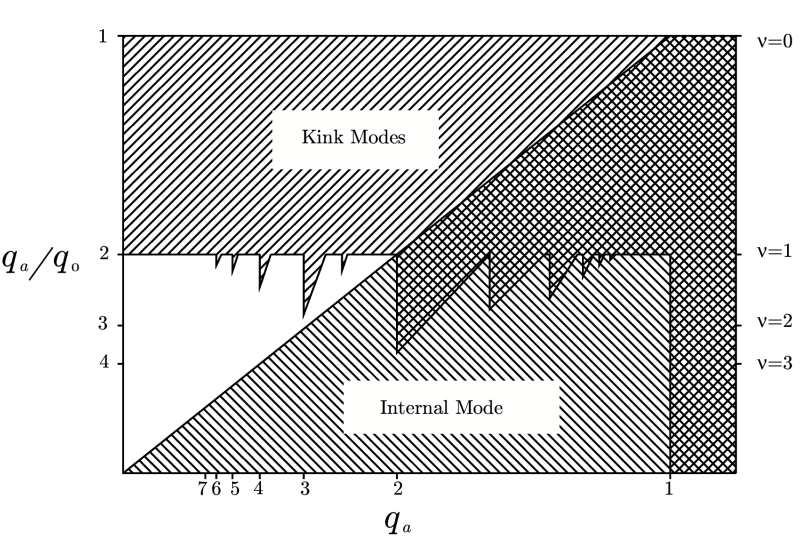
\includegraphics[width=5cm]{images/Tokamak_Stability_Diagram.png}\\



Alfven velocity: low frequency (compared to the ion cyclotron frequency) travelling oscillation of the ions and the magnetic field.  $v_{A} = B / (4 \pi n_{i} m_{i} ) ^{1/2}$.  Note $n_{i}m_{i} = \rho$\\

Lorentz Force Law: $\vec{F} = q(\vec{v}\times\vec{B} + \vec{E})$.\\  Ex: derive e and ion cyclotron frequencies from LFL: $\vec{E} \rightarrow 0$, $qvB = m\frac{v^{2}}{r}$.  $[\frac{v}{r} = \omega]$. $\frac{qB}{m} = \omega$. $[2\pi f = \omega]$. $f = \frac{qB}{2\pi m}$

Wave Stuff!\\
Propagation: R and L cutoffs:\\
$\omega_{R} = \frac{1}{2} (\sqrt{\omega_{ce}^{2} + 4 \omega_{pe}^{2}} + \omega_{ce})$\\
$\omega_{L} = \frac{1}{2} (\sqrt{\omega_{ce}^{2} + 4 \omega_{pe}^{2}} - \omega_{ce})$\\
 Upper hybrid resonance: Limit $\omega >> \omega_{ci}, \omega_{pi}$.  In this case, condition $\epsilon_{\perp} = 0$ yields:
 $\omega^{2} = \omega_{ce}^{2} + \omega_{pe}^{2}$\\
 Lower hybrid resonance: Limit $\omega << \omega_{ce}$.  In this case, condition $\epsilon_{\perp} = 0$ yields:
$\omega^{2} \approx \omega_{ci}^{2} + \frac{\omega_{pi}^{2}}{1 + \frac{\omega_{pe}^{2}}{\omega_{ce}^{2}}}$.  Say $\omega_{pe} / \omega_{ce} << 1$, underdense regime, dispersion relation becomes: $\omega^{2} \approx \omega_{ci}^{2} + \omega_{pi}^{2}$.  In case that $\omega_{pe} / \omega_{ce} >> 1$, which is known as the overdense regime, dispersion relation becomes: $\omega^{2} \approx \omega_{ce}^{2} \frac{m_{e}}{m_{i}} \approx \omega_{ce} \omega_{ci}$ 
 
The stokes diagram:\\
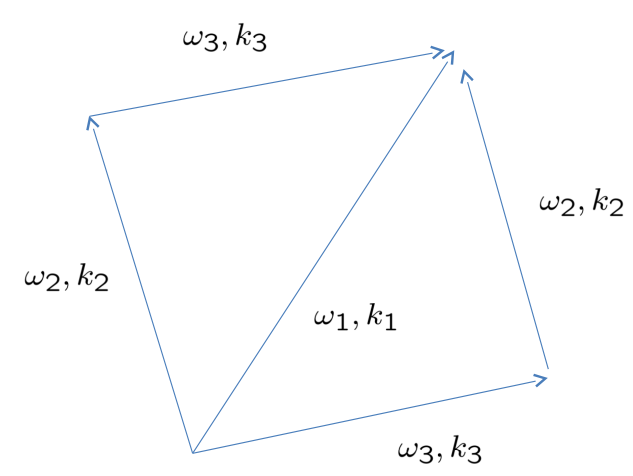
\includegraphics[width=3cm]{images/general_stokes.png}\\
Candidate waves for parametric instabilities:\\
1. Electromagnetic waves (photons):\\ $\omega^{2} = \omega_{pe}^{2} + k^{2}c^{2}$ \\
2. Electron Langmuir waves (plasmons): \\$\omega^{2} = \omega^{2}_{pe} + 3k^{2}v_{th}^{2}$\\
3. Ion sound waves (phonons): $\omega = \pm kc_{s}$\\
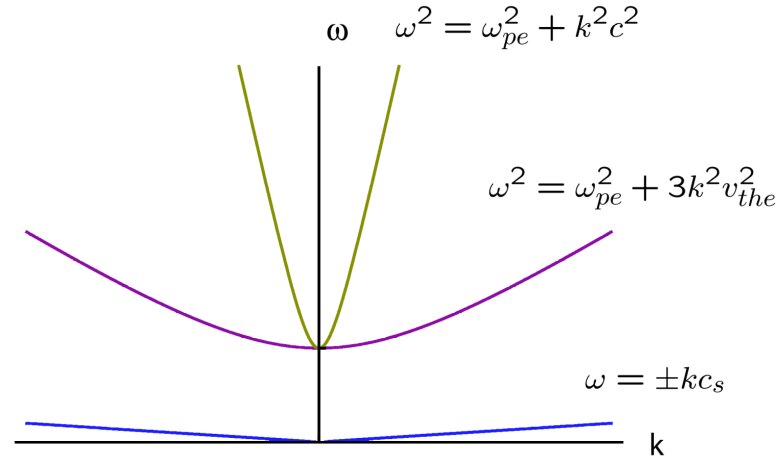
\includegraphics[width=3cm]{images/stokes_general.png}
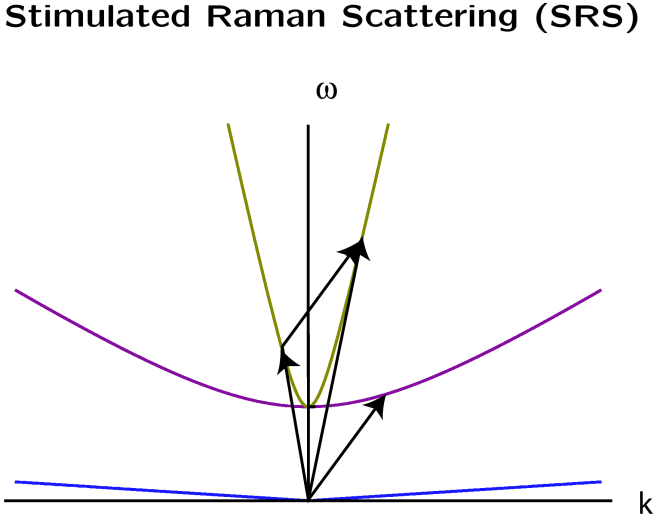
\includegraphics[width=3cm]{images/SRS.png}
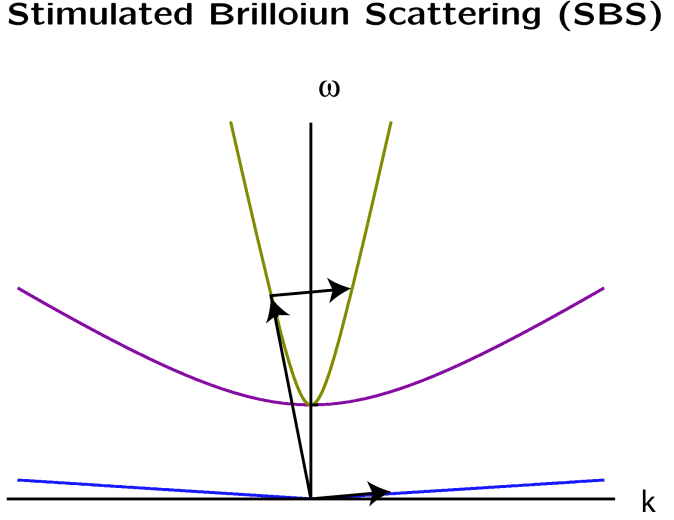
\includegraphics[width=3cm]{images/SBS.png}
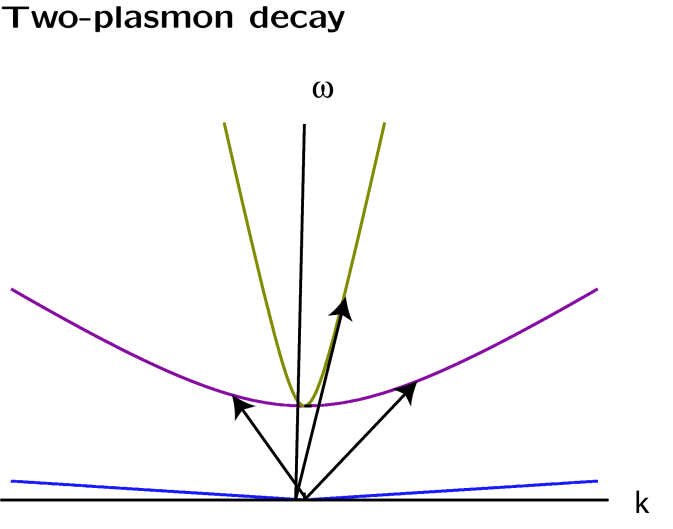
\includegraphics[width=3cm]{images/Tpd.png}


Raman and two-plasmon cases have $\omega_{2}$ and $\omega_{3} > \omega_{pe}$, so $\omega_{1}>2\omega_{pe}$.  Since $(\frac{\omega_{pe}}{\omega})^{2} = \frac{n}{n_{c}}$, where $n_{c}$ is critical density, locally $n < \frac{1}{4} n_{c}$ for these procees to occur.\\
 
Use transport equations out of plasma formulary.\\
Scaling laws for transport coefficients:  Note that for equal temps and Z=1,\\
$\frac{\tau_{i}}{\tau_{e}} \approx \sqrt{2} (\frac{m_{i}}{m_{e}})^{1/2}$ 
and so\\ 
$\frac{k_{||}^{e}}{k_{||}^{i}} \approx (\frac{3.2}{3.9})(\frac{m_{i}}{m_{e}})^{1/2} \frac{1}{\sqrt{2}}$, however:\\
$\frac{k_{\perp}^{e}}{k_{\perp}^{i}} \approx (\frac{4.7}{2})(\frac{m_{e}}{m_{i}})^{1/2} \frac{1}{\sqrt{2}}$ and the factors $\omega_{ci}\tau_{i}$ and $\omega_{ce}\tau_{e}$ are both very large.  Conclusions: Parallel transport coefficients are much greater than cross-field transport coefficients. Cross-field ion heat conduction dominates over cross-field electron heat conduction.  Parallel electron heat conduction dominates over parallel ion heat conduction.\\
Characteristic length $L = |\frac{T_{e}}{\nabla T_{e}}|$\\

Example: Parallel heat conduction: plasma at $n_{e} = 10^{20}m^{-3}$ has $1eV/m$ temp gradient at a temp of $15KeV$.  What is electron heat conduction along $\vec{B}$?  $k_{||}^{e} = 3.2\frac{nT_{e}\tau_{e}}{m_{e}}$.  $\tau_{e} = \frac{3.44 \times 10^{5}T_{e}[eV]^{3/2}}{ln(\triangle) n_{e}[cm^{-3}]} = \frac{2.0\times 10^{4} T_{e}[eV]^{3/2}}{n_{e}[cm^{-3}]} = \frac{2\times 10^{4} (15000)^{3/2}}{10^{14}} = 3.67\times 10^{-4} s$.  Now, $k_{||}^{e} = 3.2\frac{nT_{e}\tau_{e}}{m_{e}} = 3.2\frac{10^{20}(15000\times 1.6 \times 10^{-19}) 3.67 \times 10^{-4}}{9.11\times 10^{-31}} = 3.10\times 10^{32} m^{-1}s^{-1}$.  $\nabla T_{e} = 1.6\times 10^{-19} J m^{-1}$ so that $k_{||}^{e}\nabla T_{e} = 3.10 \times 10^{32} 1.6 \times 10^{-19} = 4.96 \times 10^{13} W m^{-2}$.\\
Example: Interspecies heating: D+ plasma at $n_{e} = 10^{20} m^{-3}$ with e temp 15Kev and i temp 20Kev.  What is volumetric rate of electron heating?  Note that $\tau_{e} = 3.67\times 10^{-4}s$ as before.  Then $Q_{e} = 3\frac{m_{e}}{m_{i}}\frac{n(T_{i} - T_{e})}{\tau_{e}} = 3 (\frac{9.11 \times 10^{-31}}{2 (1.67 \times 10^{-27})})10^{20}(\frac{((20,000 - 15,000)1.6\times 10^{-19})}{3.67\times 10^{-4}}) = 178kW m^{-3}$\\
Example: Cross field ion heat conduction: Ion temp near edge in D+ plasma is 1.0Kev and temp grad there is -5 kev per m. Mag field is 4T.  What is ion heat conduction there?  $k_{\perp}^{i} = 2.0 \frac{nT_{i}\tau_{i}}{m_{i}(\omega_{ci}\tau_{i})^{2}}$.  $\tau_{i} = \frac{2.09\times 10^{7} \sqrt{m/m_{p}} T_{i}[eV]^{3/2} }{ln\triangle n_{i}[cm^{-3}]} = \frac{2.09\times 10^{7} \sqrt{2} (1000)^{3/2}}{16 \cdot 10^{14}} = 5.84\times 10^{-4} s$.  $\omega_{ci} = \frac{1.6\times 10^{-19} \cdot 4}{2 \cdot 1.67 \times 10^{-27}} = 1.916 \times 10^{8} s^{-1}$.  $\omega_{ci}\tau_{i} = 1.916\times 10^{8} \cdot 5.84 \times 10^{-4} = 1.12 \times 10^{5}$.  $k_{\perp}^{i} = 2.0\frac{10^{20}\cdot 1000 \times 1.6 \times 10^{-19} \cdot 5.84 \times 10^{-4}}{2 \times 1.67 \times 10^{-27} \cdot (1.12 \times 10^{5})^{2}} = 4.47\times 10^{17} m^{-1}s^{-1}$.  $\nabla T_{i} = 5 \cdot 1.6\times 10^{-16} = 8.0 \times 10^{-16} J m^{-1}$.  $(q_{i})_{\perp} = -k_{\perp}^{i} \nabla T_{i} = 4.47 \times 10^{17} \cdot 8.0 \times 10^{-16} = 357 W m^{-2}$

 
 Collisionality:\\
 $\nu_{*} = \frac{qR}{v_{th}\tau_{i}} = \frac{\nu / \epsilon}{\omega_{b}} = \frac{\nu / \epsilon^{3/2}}{\nu_{T}/ qR} >> 1$\\
 $\nu_{i}^{*} = \frac{qR}{\nu_{th}\tau_{i}}$
 If $\nu_{i}^{*} > 1$, Pfirsch-Schutler\\
 $1 > \nu_{i}^{*} > \epsilon^{3/2}$, Plateau\\
 $\nu_{i}^{*} < \epsilon^{3/2}$.
 $\epsilon = \frac{r}{R_{0}}$\\ 
 
Ware pinch: Effect in the banana regime where trapped particles move into the plasma core under the influence of a parallel electric field. Ware pinch velocity: $\Delta v = (v_{D})_{ware} \approx \frac{cE_{\zeta}}{B_{p}}$\\ 

Rutherford island growth rate:\\
$\frac{\tau_{R}}{r^{2}} \frac{d\omega}{dt} = \Delta ^{\prime}$,
$\tau_{R}$ is the local resistive time from Spitzer resistivity,
$r$ is the minor radius at q = m/n,
$\Delta ^{\prime}$ is the classical stability index defined as the logarithmic jump of the radial magnetic field perturbation across the rational surface

$\Delta ^{\prime} > 0$ Unstable,
$\Delta ^{\prime} < 0$ Stable \\

Neoclassical correction to Rutherford growth rate:
$\frac{\tau_{R}}{r^{2}} \frac{d\omega}{dt} = \Delta ^{\prime} + \epsilon^{1/2}\frac{L_{q}}{L_{p}}\frac{\beta_{pol}}{\omega}$\\

Example: Tokamak, $B_{\theta}$ = 5.2T, $A = 3$, $q(0.9a) = 3$, $50-50DT$, circular cross section, $q=2$ surface is located at $r = 0.5a$ and $\Delta^{\prime}$ is $-50.0 m^{-1}$ there.  Answer:  At threshold value for growth, $\frac{d\omega}{dt} = 0$, $\rightarrow$  $0 = \epsilon^{\frac{1}{2}} \frac{L_{q}}{L_{p}}\frac{\beta_{pol}}{\omega}$.  $\Delta^{\prime} = \epsilon^{\frac{1}{2}} \beta_{pol} \omega$, $\rightarrow$ $\epsilon =$ inverse aspect ratio, $\beta_{pol} = \frac{-\Delta^{\prime}\omega}{\epsilon^{\frac{1}{2}}} = \frac{(50)(0.01)}{(1/3)^{1/2}} = 0.86$\\

Ara et al: (more accurate MHD gw)\\
$\gamma \tau_{A} = 0.55 (\frac{\tau_{A}}{\tau_{R}})^{3/5}(\Delta^{\prime}a)^{4/5}$\\
with: $\tau_{A} ^{-1}= \frac{B_{\theta}}{\sqrt{\mu_{0}\rho}}\frac{1}{q}\frac{dq}{dr}$
 and $\tau_{R} = \frac{\mu_{0}a^{2}}{\eta}$\\
 
 Mid Term 2 practice:\\
 1.  The ITER device $(R=6.2m,a=2.0m,B_{\phi} = 5.3T,q(0)=1.0)$ is assumed to operate with 40 MW of external heating and 80 MW of alpha-particle heating. Assume that at r = 0.9a the safety factor q is 3.0 and that the ion temperature is 3.0 keV.  Assume that the density is $8\times 10^{19}$ at this point and that the plasma is Z = 1 with a 50-50 D-T mixture.  Assume that ten percent of the heat leaves through the ion channel, neglecting ohmic heating.  Assume that both heating sources mentioned above deposit all of the heat inside the r = 0.9a surface. 
 
 (a) At r = 0.9a, find $\tau_{i}$, $\omega_{ci}\tau_{i}$ and $k_{\perp}^{i}$.  Also find the neoclassical collisionality parameter, $\nu_{i}^{*}$:  $T_{i}(0.9a) = 3000eV$.  $n_{i}(0.9a) = 8.0\times 10^{19} m^{-3} = 8.0\times 10^{13} cm^{-3}$.  $n\tau_{i} = \frac{2.09\times 10^{7}(\frac{m_{i}}{m_{p}})^{1/2}T^{3/2}_{i}}{ln(\Lambda)} = 3.61\times 10^{11} cm^{-3} s$.  $\tau_{i} = 0.0045 s$.  $\omega_{ci} = \frac{qB}{m_{i}} = 2.03 \times 10^{8}s^{-1}$. $\omega_{ci}\tau_{i} = 9.19\times 10^{5}$.  $k_{\perp}^{i} = 2.0 \frac{nT_{i}\tau_{i}}{m_{i}(\omega_{ci}\tau_{i})^{2}} = 9.80 \times 10^{16} m^{-1}s^{-1}$.  $\nu_{i}^{*} = \frac{qR}{\nu_{th}\tau_{i}} = (3)(6.2)(\frac{T_{i}}{m_{i}})^{-\frac{1}{2}} / \tau_{i} = 0.0121$.  
 
 (b)  For this value of $\nu^{*}_{i}$, find the neoclassical collisionality regime (ie Pfirsch-Schluter, Plateau or Banana:
$\nu = \frac{qR}{v_{th}\tau_{i}} = (3)(6.2)(T_{i}/m_{i})^{-1/2}/\tau_{i} = 0.0121$ so ions are Banana 
 
 
 (c) If the ion heat transport is neoclassical, find the value of $\nabla T_{i}$ at $r=0.9a$: $q^{''} = (40+80)\times 10^{6}/612 = 19,607.8 Watt m^{-2}$.  Neoclassical factor $ = Q_{neo} = 2q^{2}\epsilon^{-3/2} = 109.545$.  Since $q^{''} = -Q_{neo}k_{\perp}\frac{dT(r)}{dr}$, we have $\frac{dT(r)}{dr} = 1.8 \times 10^{-15}Jm^{-1} = 11.35keVm^{-1}$.
 
 (d) At the center of the device, the electron temperature is 25.0 keV and the ions are at 15.0 keV. The density there is $1.1\times10^{20}m^{-3}$. Find the electron-ion interspecies heating at $r=0$, in megawatts per cubic meter: $Q_{ie} = \frac{3m_{e}}{m_{i}}\frac{n(T_{i}-T_{e})}{\tau_{e}}$.  $\tau_{e} = 2.0\times 10^{10}T_{e}^{3/2}/n_{e}$ with $T_{e}$ in eV and MKS density.  Then $\tau_{e} = 718\mu s$ and $Q_{ie} = 160 kW m^{-3}$ 
 
 (e) Find the volumetric ohmic heating at $r=0$.  Give the answer in megawatts per cubic meter.  Hint: note that the toroidal current can be derived from q: $J_{\phi}(0) = \frac{2B_{\phi}(0)}{\mu_{0} q(0)R_{0}}$: $\eta = 2.8 \times 10^{-8}ZT_{e}^{-3/2} = 2.24\times 10^{-10} \Omega m$.  $J_{\phi}(0) = \frac{2B_{\phi}(0)}{\mu_{0}q(0)R_{0}} = 1.36\times 10^{6} A m^{-2}$.  $P_{\Omega} = 414.6W m^{-3}$\\
2. A hohlraum design for NIF is made with depleted uranium ($M_{u} = 238m_{p}$).  The interior of the hohlraum is illuminated with frequency-tripled neodymium-glass laser light, $\lambda = 0.35\mu$. There are two laser entrance holes (LEHs), each with a 2.0mm diameter.  The total laser power is $4.0\times 10^{14} W$ with a duration of $4.0\times 10^{-9}s$. 

(a). If the fraction of the power loss due to the blackbody radiation through the LEHs is thirty percent, find the photon temperature in the hohlraun: Radiation loss: $q^{''} = 0.3P_{laser} /A_{hole} = \frac{0.3\times4\times10^{14}}{(2(\frac{\pi d^{2}}{4	}))} = 1.91 \times 10^{15}Wcm^{-2}$. 
$q^{''}_{BB} = \sigma T_{\gamma}^{4} = 1.03 \times 10^{5}T^{4} = 1.9\times 10^{15} W cm^{-2}$.  Then, $T_{\gamma} =  (\frac{1.9\times 10^{15}}{1.03\times 10^{5}})^{1/4}$, or $T_{\gamma} = 369 eV$

(b). Assume that the electron temperature at the hohlraun wall is 3.0 keV.  Assume that the average charge $<Z>$ of the uranium is 30 and that the adiabatic index $\gamma_{e}$ for the electrons is 1.0.  Find the ion-acoustic wave speed, $c_{s}$ in the uranium plasma.  Ignore the uranium ion temperature.
The ion-acoustic wave speed is given by: 
$c_{s} = (\frac{\gamma_{e}ZT_{e} + \gamma_{i}T_{i}}{m_{i}})^{1/2}$
Using $Z=30$ and $m=238mp= 2.38 \times 1.67 \times 10^{-27}$ with $T_{e} = 3000 \times 1.6 \times 10^{-19}$ gives $c_{s} = 1.90\times 10^{5}ms^{-1}$

(c). Draw a Stokes diagram for stimulated Brillouin scattering (SBS), labeling the forward (1) and backscattered (2) electromagnetic wave and the ion acoustic wave (3).
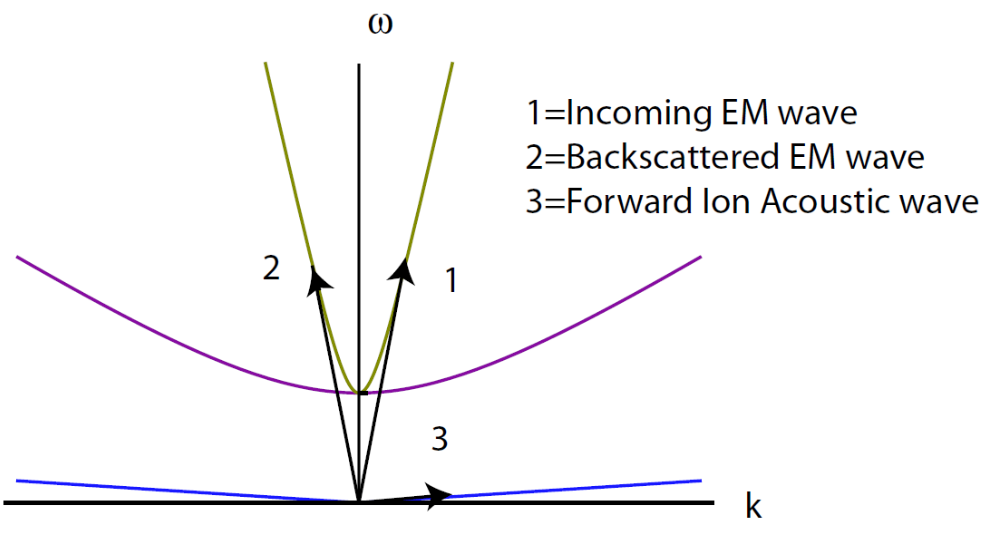
\includegraphics[width=4cm]{images/SBS_MT2.png}\\

(d). For SBS taking place where the plasma density is at 0.8x the critical density, find the value of the electron density there.
The critical density $n_{c}$ is defined as $\omega_{pe}(n_{c}) = \omega_{L}$, or $n_{c} = \frac{m_{e}\epsilon_{0}\omega_{L}^{2}}{e^{2}}$
Here $\omega_{L} = \frac{2\pi c}{\lambda_{L}} = \frac{2\pi 3\times10^{8}}{0.35\times 10^{-6}} = 5.39\times 10^{15}s^{-1}$. Then $n_{c} = 9.13 \times 10^{27} m^{-3}$ and thus $n = 0.8n_{c} = 7.31\times 10^{27} m^{-3}$

(e) Find the wavelength shift $\Delta \lambda$ for the backscattered electromagnetic wave by the following method: to first order, the wavenumber $k_{3} = 2k_{1}$.  Then find $\omega_{3} = k_{3}c_{s}$ and use this to obtain $\omega_{2} = \omega_{1} - \omega_{3}$. Then solve for the (free-space) wavelength shift using $\Delta \lambda / \lambda \approx - \Delta \omega / \omega = -\omega_{3} / \omega_{1}$.  Express your answer in angstroms. $(1\r{A} = 10^{-10}m)$
For the incoming EM wave, $\omega_{L}^{2} = \omega_{pe}^{2} + k_{1}^{2}c^{2}$
Noting that $\omega_{pe}^{2}/\omega^{2} = n/n_{c	}$ and $k_{0} = \omega/c$, this can be rewritten as $k_{1} = k_{0}\sqrt{1-n/n_{c}}$ and thus $k = \sqrt{1-0.8} \frac{2\pi c}{\lambda_{0}} = 8.03 \times 10^{6} m^{-1}$.  Then $\omega_{3} \approx 2k_{1}c_{s} = 3.056\times s^{-1}$.  Then $\Delta\omega / \omega_{L} = -5.675\times 10^{-4}$ and $\Delta\lambda = (3500)(5.675\times 10^{-4}) \r{A} = 1.98 \r{A}$

\end{multicols}
 
\end{document}